Finally, in order to ensure consistency, permanence and availability of data, MySQL server was used.
The final structure of our database can be observed in figure \ref{fig:mysql_er} and consists of the following tables:
\begin{itemize}
    \item \textbf{Admin}: Table intended to contain the information necessary to allow the admin to log in. It is not linked to any other table since there is no specific information to be maintained for this category of user 
    \item \textbf{Student}: Table intended to contain all the information needed for student login plus some personal information needed to identify the student
    \item \textbf{Professor}: Table intended to contain all the information needed for the professor's login plus some personal information needed to identify the professor
    \item \textbf{Course}: Table representing the course entity, has as foreign key the id of the professor who owns the course
    \item \textbf{Meeting\_slot}: Table intended to contain the list of weekly slots the course makes available to students. The only foreign key is used to identify the course that has made that slot available
    \item \textbf{Booked\_meeting}: Table intended to contain the list of slots booked by a student. It has two foreign keys, one needed to identify the student who booked that meeting and the other that binds the meeting to the slot of the course
    \item \textbf{Student\_starred\_course}: Table needed to keep in memory the set of courses that each student has added to favorites. It has two foreign keys, the combination of which constitutes the primary key, corresponding to the id of the student who added the course to the favorites and the id of the course 
\end{itemize}
\ \\
\begin{figure}[ht]
	\centering
	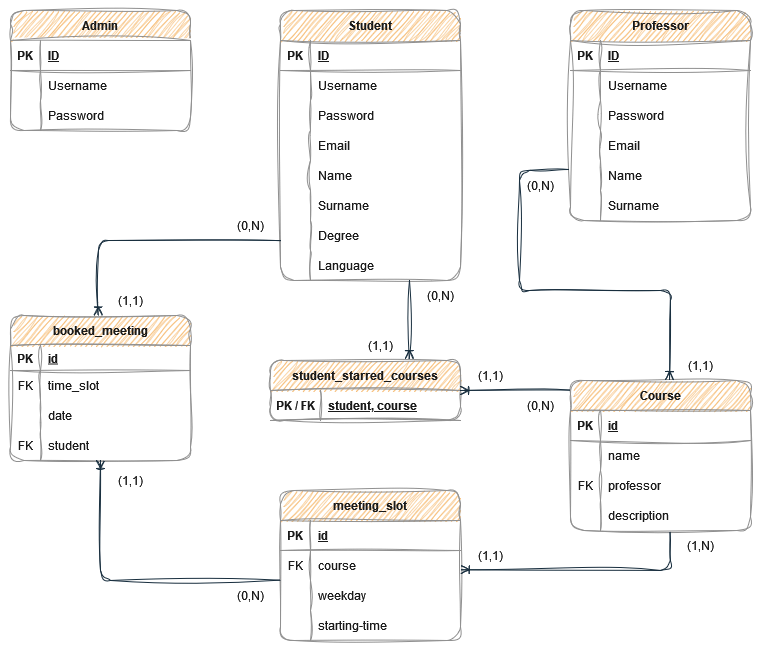
\includegraphics[width=0.8\textwidth]{img/mysql/er.png}
	\caption{Entity-Relation diagram of MySQL DB}
	\label{fig:mysql_er}
\end{figure}